\newpage
\subsection{slAdminPlugin}

La plupart des vues du lot 2 de l'Intranet d'Eyrolles sont générées grâce au plugin Symfony slAdminPlugin. Il a été développé en interne par Sensio Labs et est issu de l'abstraction du code d'un précédent projet. Il n'a rien à voir avec la fonctionnalité de génération d'administration intégrée à Symfony. C'est encore un plugin très jeune : Eyrolles est le premier projet qui l'utilise.

%format de configuration : YAML vs PHP code
%génération de code : oui non
%personnalisation de la logique : surcharge de code généré vs surcharge de méthodes d'action de base
%personnalisation des vues : surcharge de partiels générés vs écriture classique de template

Le tableau *** reprend une comparaison rapide des différences entre le moteur de génération d'administration de Symfony et slAdminPlugin. Le plugin, tout comme la génération d'administration, permet de ne pas avoir à redévelopper la logique des opérations de base, telles que le listing d'éléments, la pagination et le tri de la liste, ou encore la création, l'édition ou la suppression d'éléments. Sa valeur ajoutée est qu'il apporte plus de flexibilité quant à la personnalisation de la logique et des différentes vues.

slAdminPlugin s'articule autour de trois composants majeurs :
\begin{itemize}
\item une classe PHP de configuration ;
\item des actions d'administration de base ;
\item des widgets pour agencer la vue.
\end{itemize}

\subsubsection{La classe de configuration}

La classe de configuration permet de stocker les différents paramètres qui seront utilisés pour configurer les actions et la vue d'un module.

Une classe de configuration doit satisfaire les conditions suivantes :
\begin{itemize}
\item elle doit être placée dans le dossier \texttt{lib/config} du module et doit être nommée \texttt{slAdminConfigurationMonNomDeModule};
\item elle doit hériter de la classe abstraite \texttt{slBaseAdminConfiguration} du plugin, qui contient la liste de toutes les options disponibles ;
\item la définition des paramètres personnalisés doit se faire dans la méthode \texttt{configure()} surchargée.
\end{itemize}

Le listing *** illustre la façon d'implémenter une classe de configuration.

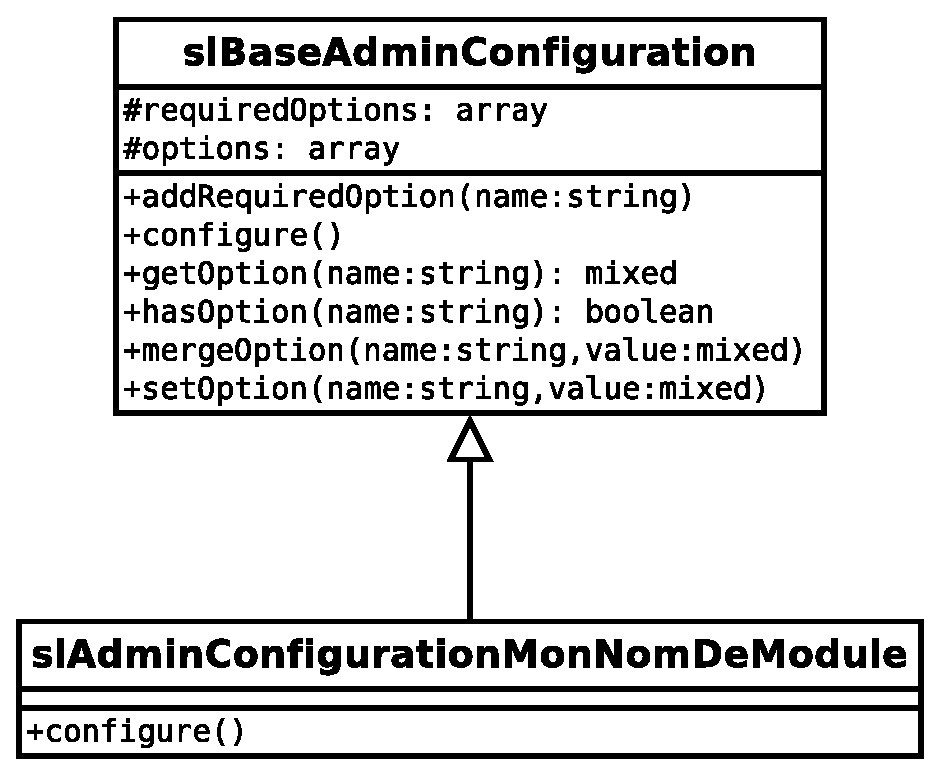
\includegraphics[]{figs/eyrolles_sladmin-config}

\subsubsection{Actions de base}

\subsubsection{Gestion de la vue}


\subsection{Un module type : le référentiel des langues}

\subsection{Utilisation de l'héritage avec Doctrine}

\subsection{Gestion de la session utilisateur avec sfGuardDoctrinePlugin}

\subsection{Export dynamique des champs des projets du panier en CSV}

\subsection{Webservice des auteurs}

\subsection{Refactoring des webservices}

\subsection{Tâche d'initialisation des auteurs}

\subsection{Refactoring des tâches}

\subsection{Écriture de tests unitaires}

\subsection{Écriture de tests fonctionnels}

\subsection{Processus de mise en production}
